\documentclass[11pt]{article}
\usepackage[margin=1in]{geometry}
\usepackage{amsmath,amssymb,amsthm,graphicx,booktabs,hyperref}
\hypersetup{colorlinks=true,linkcolor=blue,citecolor=blue,urlcolor=blue}

\newtheorem{theorem}{Theorem}
\newtheorem{lemma}{Lemma}
\newtheorem{proposition}{Proposition}
\theoremstyle{definition}
\newtheorem{definition}{Definition}
\theoremstyle{remark}
\newtheorem{remark}{Remark}

\newcommand{\R}{\mathbb{R}}
\newcommand{\E}{\mathbb{E}}

\title{Crowded Liquidation: Closed-Form Nash and Mean-Field\\
Equilibria of Optimal Execution with Permanent Impact}
\author{Anish Lotake\\ \small Independent project, November 2026}
\date{}

\begin{document}
\maketitle

\begin{abstract}
We extend the Almgren--Chriss optimal liquidation problem to $N$ symmetric traders whose
aggregate trading moves the price through linear permanent impact, and to its mean-field
limit, in the spirit of Cardaliaguet and Lehalle~\cite{CL}. Within open-loop strategies we
show that every Nash equilibrium is symmetric and solves a single linear ODE in which the
impact enters only through the effective coefficient $\alpha(1-1/N)$. This yields closed-form
equilibrium trajectories and costs, existence and uniqueness for every $\alpha\in\R$, a proof
that crowding ($\alpha>0$) strictly front-loads liquidation, a closed-form price of anarchy,
and $O(1/N)$ convergence to the mean-field limit with an explicit leading constant. All
results are verified numerically.
\end{abstract}

%=====================================================================
\section{Model}
%=====================================================================
Each of $N$ traders $i=1,\dots,N$ must liquidate an inventory $q_i(0)=Q$ by time $T$,
i.e.\ $q_i(T)=0$, trading at rate $\nu_i = q_i'$. Let $\mu(t)=\frac1N\sum_{j}\nu_j(t)$ be the
average trading rate. The mid-price, cash and objective are
\[
dS_t = \alpha\,\mu(t)\,dt + \sigma\,dW_t,\qquad
dX^i_t = -\nu_i(S_t + \kappa\nu_i)\,dt,\qquad
\max\ \E\!\left[X^i_T + q_i(T)S_T\right] - \phi\int_0^T q_i^2\,dt,
\]
with temporary impact $\kappa>0$, permanent impact $\alpha\in\R$ and risk penalty $\phi>0$.

\begin{lemma}[Deterministic reduction]
For deterministic (open-loop) strategies, trader $i$'s problem is to minimize
\[
C_i[q_i;\mu] \;=\; \int_0^T\!\big(\kappa q_i'^2 + \phi q_i^2\big)\,dt \;-\; \alpha\int_0^T q_i\,\mu\,dt .
\]
\end{lemma}
\begin{proof}
By Itô's product rule $d(q_iS)=q_i\,dS+S\,dq_i$, so
$d(X^i+q_iS) = q_i\,dS - \kappa\nu_i^2\,dt$. Integrating and taking expectations, the
$dW$ term has zero mean, giving
$\E[X^i_T+q_i(T)S_T] = X^i_0+QS_0+\alpha\!\int q_i\mu\,dt-\kappa\!\int\nu_i^2\,dt$.
Subtracting the risk penalty and dropping constants gives $-C_i$.
\end{proof}

Write $k=\sqrt{\phi/\kappa}$ and $I[q]=\int_0^T(\kappa q'^2+\phi q^2)\,dt$, the Almgren--Chriss
functional. Admissible paths are $C^1$ with $q(0)=Q$, $q(T)=0$.

%=====================================================================
\section{The single trader}
%=====================================================================
\begin{theorem}[Permanent impact is irrelevant to a lone trader]\label{thm:single}
If $N=1$ then $C_1[q]=I[q]+\tfrac{\alpha}{2}Q^2$, and the unique optimal path is
\[
q_{AC}(t) = Q\,\frac{\sinh(k(T-t))}{\sinh(kT)},\qquad I[q_{AC}] = \kappa k Q^2\coth(kT).
\]
\end{theorem}
\begin{proof}
With $\mu=q'$, $\int_0^T q q'\,dt=\big[q^2/2\big]_0^T=-Q^2/2$, a constant. $I$ is strictly
convex on the affine space of admissible paths, so its minimizer is unique and is the
solution of the Euler--Lagrange equation $\kappa q''=\phi q$ with the boundary data, which is
$q_{AC}$. For the cost, integrate by parts and use $\kappa q''=\phi q$:
$I[q_{AC}]=[\kappa q q']_0^T=-\kappa Q q_{AC}'(0)=\kappa kQ^2\coth(kT)$.
\end{proof}

%=====================================================================
\section{Nash and mean-field equilibria}
%=====================================================================
\begin{definition}
An (open-loop) Nash equilibrium is a profile $(q_1,\dots,q_N)$ such that each $q_i$
minimizes $C_i[\,\cdot\,;\mu]$ given the others' paths. A mean-field equilibrium is a path
$q$ that minimizes $C[\,\cdot\,;\mu]$ for a given $\mu$, and satisfies $\mu=q'$.
\end{definition}

\begin{lemma}[Best response]\label{lem:br}
Let $m_{-i}=\frac1N\sum_{j\neq i}\nu_j$. Player $i$'s best response is the unique solution of
$2\kappa q_i'' = 2\phi q_i - \alpha\, m_{-i}$ with the boundary data.
\end{lemma}
\begin{proof}
$C_i = \int\big(\kappa q_i'^2+\phi q_i^2-\tfrac{\alpha}{N}q_iq_i'-\alpha q_i m_{-i}\big)dt$.
The term $q_iq_i'$ integrates to a constant, so $C_i$ is strictly convex in $q_i$ and the
Euler--Lagrange equation characterizes the unique minimizer. With
$L=\kappa q'^2+\phi q^2-\tfrac{\alpha}{N}qq'-\alpha q m$:
$\partial_q L=2\phi q-\tfrac{\alpha}{N}q'-\alpha m$ and
$\tfrac{d}{dt}\partial_{q'}L=2\kappa q''-\tfrac{\alpha}{N}q'$; equating gives the claim.
\end{proof}

\begin{theorem}[Reduction to one ODE]\label{thm:ode}
Every open-loop Nash equilibrium is symmetric, $q_i\equiv q_N$, where
\begin{equation}\label{eq:ode}
q'' + a\,q' - k^2 q = 0,\qquad q(0)=Q,\ q(T)=0,\qquad a = a_N := \frac{\alpha}{2\kappa}\Big(1-\frac1N\Big).
\end{equation}
The mean-field equilibrium solves the same problem with $a=a_\infty:=\alpha/(2\kappa)$.
\end{theorem}
\begin{proof}
\emph{Symmetry.} For $i\neq j$ let $d=q_i-q_j$. Since $m_{-i}-m_{-j}=(\nu_j-\nu_i)/N=-d'/N$,
Lemma~\ref{lem:br} gives $2\kappa d''-\tfrac{\alpha}{N}d'-2\phi d=0$ with $d(0)=d(T)=0$. The
characteristic roots are real and distinct (discriminant $\alpha^2/N^2+16\kappa\phi>0$), and
the only such solution vanishing at both ends is $d\equiv0$.
\emph{Equation.} With all paths equal, $m_{-i}=\tfrac{N-1}{N}q'$; substituting into
Lemma~\ref{lem:br} and dividing by $2\kappa$ gives \eqref{eq:ode}.
\emph{Mean field.} The best response to a given $\mu$ is $2\kappa q''=2\phi q-\alpha\mu$
(Lemma~\ref{lem:br} with $m_{-i}$ replaced by $\mu$, the own-impact term vanishing in the
limit). Imposing $\mu=q'$ gives \eqref{eq:ode} with $a_\infty$.
\end{proof}

\begin{remark}
A trader's own share $\tfrac1N$ of the impact drops out because it only contributes a
boundary term. Equilibrium is therefore governed by the impact of \emph{others}, which is why
$N=1$ recovers Almgren--Chriss (Theorem~\ref{thm:single}).
\end{remark}

\begin{theorem}[Closed form, existence and uniqueness]\label{thm:closed}
For every $\alpha\in\R$ and $N\in\{1,2,\dots\}\cup\{\infty\}$, \eqref{eq:ode} has the unique solution
\[
q_N(t) = Q\,e^{-a t/2}\,\frac{\sinh(\omega(T-t))}{\sinh(\omega T)},\qquad
\omega=\omega_N=\sqrt{a^2/4+k^2}>0,
\]
with cost $I[q_N] = \kappa\,\omega\, Q^2\coth(\omega T)$.
\end{theorem}
\begin{proof}
Put $q=e^{-at/2}u$. Then $q''+aq'-k^2q=e^{-at/2}\big(u''-\omega^2u\big)$, so $u''=\omega^2u$,
whose general solution is $A\sinh(\omega(T-t))+B\sinh(\omega t)$. The boundary data give
$A\sinh(\omega T)=Q$ and $B\sinh(\omega T)=0$. Since $\omega>0$, $\sinh(\omega T)\neq0$, so
$A,B$ are uniquely determined ($B=0$). This holds for every real $a$, hence every $\alpha$.
For the cost, integrate $\int\kappa q'^2$ by parts and use $\kappa q''=\phi q-\kappa a q'$:
$I[q]=-\kappa Qq'(0)-\tfrac{\kappa a}{2}Q^2$. With
$q'(0)=-Q\big(\tfrac a2+\omega\coth(\omega T)\big)$ this equals $\kappa\omega Q^2\coth(\omega T)$.
\end{proof}

%=====================================================================
\section{Crowding: front-loading and inefficiency}
%=====================================================================
\begin{lemma}\label{lem:h}
$h(x)=x\coth x$ is strictly increasing on $(0,\infty)$.
\end{lemma}
\begin{proof}
$h'(x)=\dfrac{\sinh x\cosh x-x}{\sinh^2x}=\dfrac{\tfrac12\sinh(2x)-x}{\sinh^2x}>0$, since $\sinh y>y$ for $y>0$.
\end{proof}

\begin{theorem}[Crowding front-loads liquidation]\label{thm:front}
If $\alpha>0$ and $N\geq2$ (including $N=\infty$), then $q_N(t)<q_{AC}(t)$ for all $t\in(0,T)$.
\end{theorem}
\begin{proof}
Here $a>0$ and $\omega>k$. With $s=T-t\in(0,T)$,
\[
\frac{q_N(t)}{q_{AC}(t)} = e^{-at/2}\cdot\frac{g(\omega)}{g(k)},\qquad g(w)=\frac{\sinh(ws)}{\sinh(wT)}.
\]
The first factor is $<1$. For the second,
$\frac{d}{dw}\log g = s\coth(ws)-T\coth(wT)=\tfrac1w\big(h(ws)-h(wT)\big)<0$ by
Lemma~\ref{lem:h}, so $g(\omega)<g(k)$.
\end{proof}

\begin{remark}
For $\alpha<0$ the factor $e^{-at/2}$ exceeds $1$ while $g(\omega)/g(k)$ is still below $1$, so
the two effects compete. Numerically (Section~\ref{sec:num}) the exponential dominates for
every tested $\alpha\in[-1.5,0)$ and liquidation is \emph{back}-loaded; a proof is left open.
\end{remark}

\begin{theorem}[Inefficiency of equilibrium]\label{thm:poa}
\begin{enumerate}
\item A social planner minimizing total cost $\sum_iC_i$ assigns every trader $q_{AC}$.
\item The equilibrium excess cost $\Delta_N = I[q_N]-I[q_{AC}]\geq0$ for all $\alpha\in\R$,
with equality iff $N=1$ or $\alpha=0$.
\item For $\alpha\geq0$, the price of anarchy is
\[
\mathrm{PoA}(\alpha,N)=\frac{C[q_N]}{C[q_{AC}]}
=\frac{\kappa\omega_N\coth(\omega_NT)+\alpha/2}{\kappa k\coth(kT)+\alpha/2}\;\geq\;1.
\]
\end{enumerate}
\end{theorem}
\begin{proof}
(1) $\sum_iq_i\mu=N\bar q\,\bar q'$ with $\bar q=\frac1N\sum q_i$, and $\bar q(0)=Q$,
$\bar q(T)=0$, so $\sum_iC_i=\sum_iI[q_i]+\tfrac{\alpha N}{2}Q^2$. Each $I[q_i]$ is minimized
by $q_{AC}$ (Theorem~\ref{thm:single}).
(2) By Theorems~\ref{thm:single} and~\ref{thm:closed}, $I[q_N]=\tfrac{\kappa Q^2}{T}h(\omega_NT)$
and $I[q_{AC}]=\tfrac{\kappa Q^2}{T}h(kT)$. Since $\omega_N\geq k$ with equality iff $a_N=0$,
Lemma~\ref{lem:h} gives the claim.
(3) In a symmetric profile $\mu=q'$, so each trader pays $C=I[q]+\tfrac\alpha2Q^2$; divide and
use (2). For $\alpha\geq0$ the denominator is positive so the ratio is meaningful.
\end{proof}

\begin{remark}
For sufficiently negative $\alpha$ (here $\alpha<-2\kappa k\coth(kT)\approx-0.63$) total costs
become negative and the ratio loses meaning; the excess cost $\Delta_N$ is the right measure.
\end{remark}

%=====================================================================
\section{Convergence to the mean-field limit}
%=====================================================================
\begin{theorem}[$O(1/N)$ convergence with explicit constant]\label{thm:conv}
Write $q(t;a)$ for the solution in Theorem~\ref{thm:closed}. Then
\[
\big\|q_N-q_\infty\big\|_\infty = \frac{|\alpha|}{2\kappa N}\,\big\|\partial_a q(\cdot;a_\infty)\big\|_\infty + O(N^{-2}),
\]
where
$\partial_a q(t;a) = q(t;a)\Big[-\tfrac t2+\tfrac{a}{4\omega}\big((T-t)\coth(\omega(T-t))-T\coth(\omega T)\big)\Big]$.
\end{theorem}
\begin{proof}
$a_N-a_\infty=-\alpha/(2\kappa N)$. The map $(t,a)\mapsto q(t;a)$ is smooth on
$[0,T]\times\R$ (the bracket extends continuously to $t=T$), so Taylor's theorem in $a$ with
$\partial_a^2q$ bounded on the compact set $[0,T]\times[a_N,a_\infty]$ gives
$q_N-q_\infty=(a_N-a_\infty)\partial_aq(\cdot;a_\infty)+O(N^{-2})$ uniformly in $t$. The formula
follows from $\partial_a\log q=-\tfrac t2+\tfrac{d\omega}{da}\big((T-t)\coth(\omega(T-t))-T\coth(\omega T)\big)$
and $d\omega/da=a/(4\omega)$.
\end{proof}

%=====================================================================
\section{Numerical verification}\label{sec:num}
%=====================================================================
Parameters: $T=Q=1$, $\kappa=0.1$, $\phi=1$ (so $k=\sqrt{10}$). Code: \texttt{src/mfg.py}.

\begin{table}[h]\centering
\begin{tabular}{@{}lll@{}}\toprule
Check & Result & Theorem\\\midrule
Closed form vs.\ \texttt{solve\_bvp}, $\alpha\in[-1.5,5]$, $N\in\{1,2,10,100,\infty\}$ & max rel.\ error $5.8\times10^{-14}$ & \ref{thm:closed}\\
$q_1 = q_{AC}$ & difference exactly $0$ & \ref{thm:single}\\
Inventory sold by $T/2$: AC / $\alpha{=}1$ / $\alpha{=}5$ / $\alpha{=}{-1}$ & $80.3\%$ / $96.2\%$ / $\approx100\%$ / $54.3\%$ & \ref{thm:front}\\
PoA$(\alpha,\infty)$ at $\alpha=1,\,2,\,5$ & $1.105,\ 1.208,\ 1.345$ & \ref{thm:poa}\\
Fitted slope of $\log\|q_N-q_\infty\|_\infty$ vs.\ $\log N$, $N\in[10,10^4]$ & $-1.002$ & \ref{thm:conv}\\
$N\|q_N-q_\infty\|_\infty$ at $N=10^6$ vs.\ predicted constant ($\alpha=1$) & $0.2272876$ vs.\ $0.2272875$ & \ref{thm:conv}\\
\bottomrule\end{tabular}
\end{table}

\begin{figure}[h]\centering
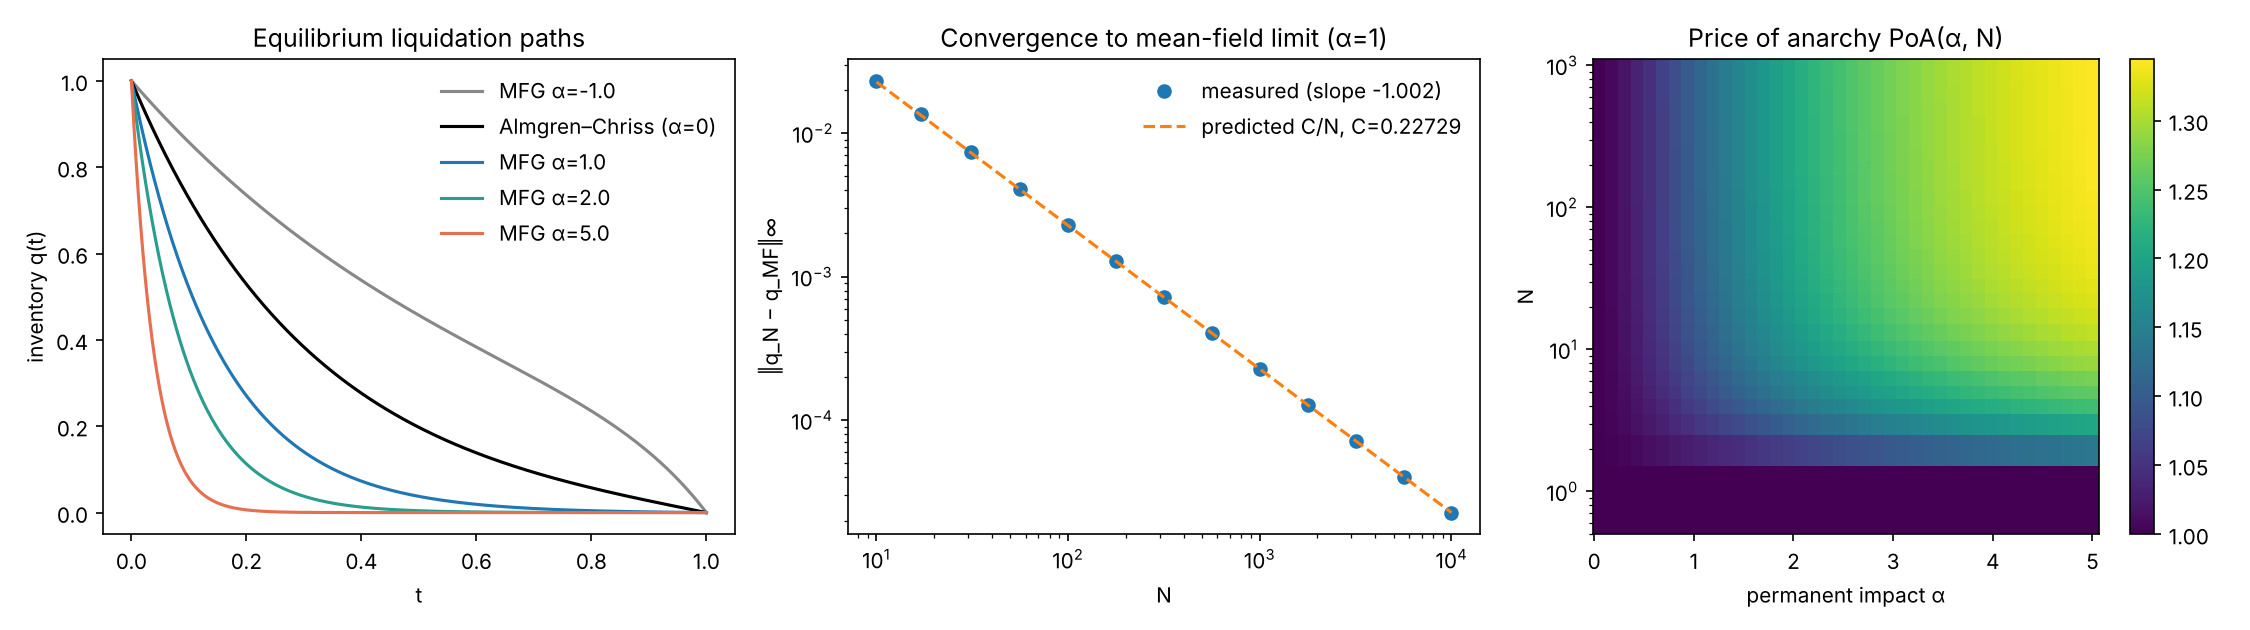
\includegraphics[width=\textwidth]{../figures/mfg_results.png}
\caption{Left: equilibrium paths; crowding ($\alpha>0$) front-loads, $\alpha<0$ back-loads.
Centre: $O(1/N)$ convergence, measured vs.\ predicted constant. Right: price of anarchy.}
\end{figure}

%=====================================================================
\section{Limitations and extensions}
%=====================================================================
Strategies are open-loop and deterministic; closed-loop (feedback) Nash equilibria of the
$N$-player game generally differ at finite $N$ and are characterized by coupled Riccati
equations. Impact is linear and traders are homogeneous. Natural extensions are heterogeneous
initial inventories, which lead to a forward--backward ODE for the mean inventory as in~\cite{CL},
and a proof of back-loading for $\alpha<0$.

\begin{thebibliography}{9}
\bibitem{AC} R.~Almgren and N.~Chriss. Optimal execution of portfolio transactions.
\emph{Journal of Risk}, 3(2):5--39, 2001.
\bibitem{CL} P.~Cardaliaguet and C.-A.~Lehalle. Mean field game of controls and an
application to trade crowding. \emph{Mathematics and Financial Economics}, 12:335--363, 2018.
\end{thebibliography}

\end{document}
